\section{Microarchitectural Timing Channels}

This section discusses internal timing channels in typical
multi-core processors and mechanisms to control them.

\subsection{Baseline Architecture}

    \begin{figure}
        \begin{center}
            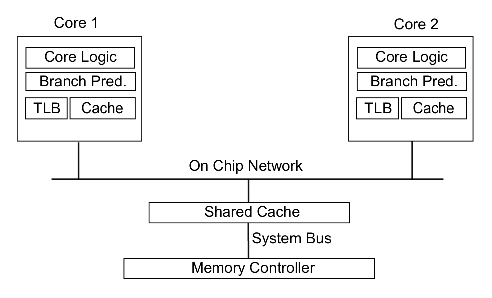
\includegraphics[width=3.04in]{figs/baseline.eps}
            \caption{Baseline multi-core architecture.}
            \label{fig:baseline}
        \end{center}
    \end{figure}

Figure \ref{fig:baseline} shows a baseline multi-core architecture that we
extend with timing compartments in this paper. The architecture
has multiple cores, each with a core pipeline, a branch predictor, a TLB,
and one or more private caches. 
The cores are connected to a shared cache via an on chip network. A shared system 
bus connects the shared cache to a memory controller that manages requests to 
main memory.
We assume that each core may be time shared by multiple timing
compartments, but only one timing compartment, which we say is active, may run each core
at a time. This assumption can be relaxed if timing channel protection
is added to per-core resources.

%A trusted software layer (such as 
%an operating system) allocates software entities (such as processes) to the 
%cores. 

\subsection{General Protection Approaches}

Here, we present a classification of internal microarchitectural timing channels 
and a framework of general solutions to address each type.
We follow these approaches to design our
protection mechanisms. These approaches also provide guidelines to
develop new protection mechanisms for components that are not included in
our baseline architecture.

\subsubsection{Classification of Internal Timing Channels}

There exists an internal timing channel from one entity (say $E1$)
to another ($E2$) whenever the timing of an action of $E1$ can be affected 
by the behavior of $E2$.

There are two types of such timing channels in hardware: state-based
and contention-based.
A \emph{state-based} timing channel occurs whenever there is a state element 
with an access time that depends on its content and that state element is 
shared among multiple entities.
For example, a conventional shared cache has state-based timing channels, because 
its cache hits are faster than misses.
A \emph{contention based} timing channel occurs whenever multiple entities 
share a resource that can handle only finitely many requests at a time.
Conventional buses have contention-based timing channels.

\subsubsection{State-Based Timing Channel Protection}

%Caches, TLBs, and branch predictors all have state-based timing channels. 
%In 
%each, requests that use an entry that is present in the state elements (e.g.  
%cache hits) are faster than requests to entries not present (e.g. cache 
%misses). The state elements can contain a finite number of entries, so entries 
%must be evicted and replaced with new ones. One software entity can evict 
%entries owned by another, causing interference and timing channel leakage if 
%the choice of entries evicted correlates with a secret. 
In general, the state-based 
timing channels can be removed by applying flattening, partitioning, or 
flushing.
Flattening eliminates the dependence of access time on the state by forcing 
every access to finish in the same (worst case) time. For example, to remove timing 
interference in the row buffers of DRAM, all DRAM accesses may be treated as 
a row buffer miss.
For some components, this is a 
brute-force approach. Applied to caches, every access must be treated as a 
miss, so this is equivalent to removing the cache. 

Partitioning removes interference by ensuring that each entity can
only affect a disjoint subset of state elements. The partitions
should not change dynamically depending on the run-time demands of entities.
In the simplest case, partitions can be static.
However, partitions do not need to be heterogeneous and can be sized according 
to static performance characterizations of each software entity (assuming this 
information can be made public and does not depend on secrets).

%prevents software entities that share state elements from 
%interfering. Static partitioning is realized by dividing the state elements 
%into separate partitions for each software entity. Entities are only allowed to 
%evict entries within their own partitions. Partitions must either be static, or 
%at least not resized or moved based on the dynamic behaviour of an entity.
%% If a partition is increased for an entity intensively using the state 
%% elements, the other entities can detect that their partitions have been 
%% resized and information is leaked.
%However, partitions do not need to be heterogeneous and can be sized according 
%to static performance characterizations of each software entity (assuming this 
%information can be made public).

Flushing can remove state-based timing channels for a resource that is time-shared.
For example, a branch prediction table may be cleared on a context switch.
%At the end of a time quantum, the state elements are completely cleared before 
%passing ownership of the state elements to the entity in the next time quantum.  
%Resources that can be flushed can also be partitioned, and there are tradeoffs 
%between these approaches.
% Flushing increases the time wasted at the end of a time quantum if flushing 
% cannot be done in less than one clock cycle. Clearing the state between time 
% quanta also increases the number of slower accesses at the start of the 
% quanta (e.g. it causes more cold cache misses). However, partitioning reduces 
% the total number of state elements that can be allocated to each entity. 
In general, there is a trade-off between partitioning and flushing.
For long time slices (e.g. when context switching is infrequent), 
flushing is preferable because it allows the full capacity to be used by
each timing compartment. In contrast, partitioning may
offer better performance for short time slices by reducing cold misses.
%time to reload
%the state on a context switch.

\subsubsection{Contention-Based Timing Channel Protection}

%Contention based timing channels arise whenever a resource that is shared among 
%multiple software entities can only handle a finite number of requests at a 
%time. 
Contention based timing channels can be removed by duplication or by
time division multiplexing (TDM). Duplication removes interference by
allocating dedicated resources for each timing compartment.
However, this has obvious area overhead implications. If 
duplication is infeasible, time division multiplexing can be used.
%TDM 
%defines a schedule where each software entitiy is guaranteed a period of time, 
%called a time quantum, where only that entity can use the resource. The 
The schedule of time slices must either be static or independent of the 
dynamic behavior of software entities.

%\subsubsection{External Timing Channel Protection}
%
%Though external timing channels are outside the scope of this 
%paper, there are a class of timing channels that are internal to hardware, but 
%appear as external timing channels between two software entities. This form of 
%external timing channel exists in systems where distrusting software entities 
%must communicate. For example, one software entity might be a user space 
%process and another might be a process that performs only high-assurance 
%operations. The user space process requests the high-assurance process to 
%perform some operation on its behalf. The user space process can directly 
%observe the execution time of the other process. This type of timing channel 
%can be solved in software by forcing the observable execution time to 
%equal the worst case execution time, stalling if necessary.


\subsection{Full-Processor Protection}

Timing compartments use hardware mechanisms that control all internal timing 
channels in a microprocessor. Designing a full processor with timing channel
protection may seem rather straightforward. In our baseline architecture, there are
only three main structures that are shared concurrently: a shared cache, on-chip
buses, and a memory controller. Moreover, recent studies have proposed mechanisms
to control timing channels in each of them. For example, researchers have proposed
statically partitioning the shared cache \cite{percival}, and using time division 
multiplexing with a fixed schedule for the on-chip interconnect 
\cite{yaonocs, surfnoc} and the memory controller \cite{ushpca14}.

%Many microarchitectural timing channels and corresponding solutions are 
%well-known. Shared caches create a state-based timing channel where interfering 
%entities cause cache block replacements. This can be prevented by partitioning 
%the cache among the entities. On chip networks and buses have
%timing channels since only one entity can use the bus at a time. Time division 
%multiplexing can resolve this issue \cite{yaonocs}. The authors of 
%\cite{ushpca14} have exposed timing channels in the main memory and memory 
%controller. They propose time division multiplexing the memory controller, 
%partitioning the memory controller queueing structure, and using a closed-page 
%row buffer management policy to close these timing channels. 
%%%%% It isn't totally obvious that private resources are actually shared, and 
%%%%% we don't have a citation for this, so maybe it doesn't need to be here..
% Finally, the private, per-core resources of the system such as the branch 
% predictors, TLBs and private caches also create timing channels since 
% software entities share cores through time multiplexing (for example, 
% processes may be context switched in and out of the same core). These can be 
% resolved by flushing the state elements of these resources on before moving a 
% new software entity onto the core.

However, achieving secure and efficient timing channel protection on a full processor
requires much more than simply putting known protection mechanisms
together. During the design process, we found three new sources of timing channels
in module interfaces that were not discussed previously, and found a bug in the
memory controller protection \cite{ushpca14}.
%The cache protection scheme also needed to be slightly changed to handle cases when timing
%compartments have shared memory pages. 
We also found that time multiplexed
microarchitecture structures must be carefully coordinated in order to avoid 
unnecessarily high overheads. 
%%%%% We have not demonstrated total starvation in practice or on paper.
% or total starvation.

The rest of this section provides a detailed list of timing channels in our
baseline architecture, and presents a protection mechanism that we use for each of them.
Table \ref{table:timing_chan_summary} summarizes these timing channels and
solutions. 
Then, the next section discusses how these protection mechanisms
need to be managed and coordinated together.
We note that the processor design here uses simple static protection
mechanisms that prevent timing channels in both directions. The mechanisms 
can be further optimized for efficiency.

\def\novelcolor{Green}
\begin{table*}
\begin{tabular}{l|l|l|l}
    \hline
    Component & Timing Channel & Classification & Solution\\
    \hline
    \multirow{3}{*}{Shared Caches}
    & Replacement & State  & Set Partitioning \\
    \hhline{~---}
    & {\color{\novelcolor}MSHRs}
    & {\color{\novelcolor}Contention }
    & {\color{\novelcolor}Duplicate MSHR Banks} \\
    \hhline{~---}
    & {\color{\novelcolor}Response Ports}
    & {\color{\novelcolor}Contention }
    & {\color{\novelcolor}Separate Queues \& Time Multiplexing}\\
    \hline
    \multirow{5}{*}{DRAM \& Memory Controller}
    & Page Faults & State  & Address Space Partitioning \\
    \hhline{~---}
    & DRAM Resources & Contention  & Time Multiplexing \\
    \hhline{~---}
    & Queueing Structure & State  & Partitioned Queue \\
    \hhline{~---}
    & Row Buffer & State & Closed Page Policy (Flattening)\\
    \hhline{~---}
    & {\color{\novelcolor} Response Ports} 
    & {\color{\novelcolor} Contention }
    & {\color{\novelcolor} Separate Queues \& Time Multiplexing}\\
    \hline
    \multirow{2}{*}{Network} 
    & Interconnect Contention & Contention & Time Multiplexing \\
    \hhline{~---}
    & Queueing Structure & State & Partitioned Queue \\
\end{tabular}
    \caption{Summary of timing channels and protection approaches. Green represents new timing channels that were not identified in previous work.}
    \label{table:timing_chan_summary}
\end{table*}

\subsubsection{Shared Caches}
\mbox{}\newline
\textbf{Cache State \& Replacement}
The shared cache causes state-based timing channel vulnerabilities, because accesses
from one timing compartment may evict the cache blocks of another timing compartment.
This state-based timing channel is the focus of prior cache timing channel 
studies.
%to the memory hierarchy for addresses that are stored in the cache (cache hits) 
%are returned faster than requests for entries not stored in the cache (cache 
%misses). So, the time required to access the cache depends on its state. The 
%cache can only accommodate a finite number of entries, so when new entries must 
%be stored, old ones are evicted. One software entity can evict the entries of 
%another, causing timing channel leakage.

Our design uses static cache partitioning to eliminate the cache
interference among timing compartments.
The cache state of different timing compartments are forced to reside in 
disjoint regions of the cache so that one timing compartment cannot evict the 
entries of another.
In general, there exist two approaches for cache partitioning:
way partitioning \cite{dynamic_partitioning} and
set partitioning \cite{rtas_cache_framework}. Way partitioning restricts
each compartment to only replace certain cache ways. Set partitioning
either uses page coloring or modifies the index function so that each compartment
only uses a subset of the cache sets. Both partitioning methods are equally
effective at removing timing channels. In our implementation, we used
set partitioning so that each compartment can benefit from full 
cache associativity.

%We note that the cache partitioning needs a special care if multiple timing
%channels shared the same physical memory location. In this case, a cache
%access from one compartment may hit in another compartment partition. Such a
%hit must be handled as a miss from the timing perspective. 


%Set associative caches divide 
%the cache into ways. Each way as a single slot for each cache set. A cache 
%block may be stored in any way, but the set it belongs to is determined by a 
%segment of its address bits called the index. Since many addresses are mapped 
%to the same set, another segment of the address, the tag, is used to detect 
%cache hits (i.e. if a specific address is present in the cache).

%Way partitioning allocates a subset of the ways to each entity 
%\cite{citation_needed}. This results in a reduction in the effective 
%associativity utilized by each entity, and thus, causes more conflict misses 
%and weakens performance. Set partitioning manipulates virtual to physical 
%address translation to restrict the sets that a particular entity can occupy.  
%When done at the granularity of a page, this is called page coloring, and this 
%has been proposed for performance \cite{citation_needed} and real-time systems 
%\cite{rtas_cache_framework}.  Although both techniques increase the number of 
%capacity misses, set partitioning does not increase the number of conflict 
%misses, so we chose this technique for our implementation.

\textbf{MSHR Contention}

We identified new internal timing channel vulnerabilities in the shared cache 
interface. The first, is caused by contention for the miss status holding 
registers (MSHRs) in non-blocking caches.
A non-blocking cache uses MSHRs to track information about in-flight cache misses 
(memory requests).
% With only a single MSHR, the system can tolerate a single outstanding cache 
% miss (hit under miss). With more MSHRs, it can tolerate multiple outstanding 
% misses (miss under miss). In any case, the system can tolerate only finite 
% outstanding misses at a time. 
The number of outstanding cache misses that the cache can tolerate depends on 
the number of MSHRs. Once all MSHRs are exhausted, the cache will stall on
a miss resulting in increased latency for cache accesses.
Therefore, shared MSHRs cause an internal timing channel, because one timing
compartment can delay accesses from another compartment by exhausting the MSHRs.
To remove the MSHR contention timing channel, our processor design duplicates
the MSHRs and dedicates MSHRs to each timing compartment.

\textbf{Response Port Contention}
The cache ports cause another contention-based timing channel yet to be 
discussed in the literature. Conventional caches have CPU-side ports and 
memory-side ports both of which are split into request and response ports. 
%On the cache miss path, the cache receives a request through the CPU-side request 
%port, and detects a miss. The cache issues a request to the memory through its 
%memory-side request port and then receives a response through its memory-side 
%response port. Finally, the cache responds to the CPU through its CPU-side 
%response port.
However, each port can only service a single response/request at a time
causing contention for these ports. For example, in a non-blocking cache,
data from an outstanding miss may be ready while a response for a cache hit
is being transferred through the CPU-side port.
It is also possible that the CPU-side bus is busy and will block the response
port. 
%Requests to the cache are controlled through the on 
%chip network, so any contention for this port may be controlled there. However, 
%there is uncontrolled contention in the CPU-side response port. Typically cache 
%accesses return more data than can be sent over a bus in a single cycle, 
%necessitating multi-cycle transfer (for example a cache block may consist of 
%several words and the bus may allow only a single word to be transferred each 
%bus cycle). Since the cache is nonblocking, it is possible for a response from 
%memory to return to the cache and require the cache response port while the 
%data from a cache hit is being transferred. 
To deal with this port contention, conventional caches include a shared queue
where responses can be buffered. Unfortunately, 
timing interference in either the cache ports or the cache response queue can
lead to an internal timing channel. To remove this timing channel, we apply
time division multiplexing to the cache ports and replace a shared queue with
smaller per-compartment queues.

\subsubsection{On-Chip Interconnect}

As pointed out by previous studies \cite{yaonocs, surfnoc}, shared on-chip 
interconnects
have contention-based timing channels because each link can be used by only 
one compartment at a time. If the network contains buffers, they also lead
to state-based timing channels. In our processor design, we apply time
division multiplexing with a fixed schedule to both the bus between private
and shared caches and the bus between the shared cache and the memory controller.
For each time slice, accesses from only one timing compartment are allowed to
use the bus.

\subsubsection{Main Memory Controller}

The main memory is shared concurrently among multiple cores. As a result,
interference among memory accesses from multiple timing compartments can lead
to internal timing channels. 
%and 
%analogous to the timing disparity between cache hits and misses, page faults in 
%main memory take substantially longer than accessing entries that are present 
%in main memory. This timing channel can be handled simply by partitioning the 
%address physical address space for each entity.
%However, the memory controller has additional timing channels due to resource 
%contention as well as other state based timing channels. 
Wang et al. proposed a timing channel protection scheme for the shared memory
controller, which is based on time division multiplexing \cite{ushpca14}. 
We adopt their protection scheme in our processor design and briefly summarize 
the sources of timing interference and countermeasures here.
However, we found a minor vulnerability in their protection scheme and
adjusted the scheme to remove it.

\textbf{Request Queue}
A conventional memory controller has a queue for buffering memory requests until
they can be issued. This queue is typically shared among requests and creates
a state-based timing channel, because requests from one compartment can block
requests from another. We remove this interference by placing the shared 
queue with smaller per-compartment queues, effectively partitioning the single queue.

\textbf{Row Buffer State}
There exists another state-based timing channel in the shared memory controller
if an open page policy is used. On a DRAM access, an entire row is read from
a memory array and stored in a row buffer (sense amplifier). If this buffer is
used as a cache, it creates a timing channel, because consecutive accesses to 
the same row are faster than accesses to different rows.
The protection scheme removes this timing channel by applying the closed page
policy, which precharges the row buffer after each access. This
closed page policy can be seen as an application of the flattening approach that
treats each access as a row buffer miss.
A previous study \cite{ushpca14} showed that the close page policy does
not have a noticeable performance disadvantage over the open page policy, because it
makes an access to a different row faster by performing a precharge early.

\textbf{DRAM Contention}
The DRAM device contains several resources such as the command bus, data
bus, banks, and ranks that can only service a finite number of requests at a time. 
Therefore, these cause contention-based timing channels.
%For example, two requests to the same bank cannot
%be scheduled at the same time. In a conventional memory controller, one request 
%would be delayed, causing interference.
% Suppose the queueing structure contains a request from a victim owned 
% software module for a bank. If an adversarial software module issues a 
% request to the same bank, it will be delayed, informing the adversary that 
% such a victim request exists. Similarly, contention for the command bus 
% causes a timing channel that may be observed in the scheduler. If a request 
% from one software module arrives at the scheduler in the same cycle as a 
% request from another software module and for a different bank, one of the 
% requests is scheduled and the other is delayed since only a single command 
% can occupy the command bus at a time.
The protection scheme uses timing division multiplexing (TDM) to remove these
timing channels. The TDM protection for main memory requires a special period 
in each time slice where no new
request can be issued in order to prevent in-flight requests or refreshes to
create timing interference.

%A surprising contention timing channel due to refreshes complicates TDM for 
%memory controllers. DRAM banks that are handling a request cannot be refreshed, 
%so refreshes are actually stalled by regular requests. This stall can shift the 
%refresh to the following turn and indicate that an access to that bank is 
%taking place. Since the refresh timing is public information, the dead time of 
%each time quantum where a refresh takes place is increased to guarantee the 
%refresh completes.

\textbf{Adjustments to the Protection Scheme}
During the process of integrating timing protection mechanisms for a full
processor, we found two vulnerabilities in the previously proposed scheme.
First, similar to the shared cache, the response port of a memory controller
can lead to a contention-based timing channel. We removed this channel by
separating queues for each timing compartment and applying TDM to the port.
Second, we found that the dead time proposed by ~\cite{ushpca14} was 
not sufficiently long. Previous work erroneously assumed that requests to two
different ranks would not interfere.

\subsubsection{Private Per-Core Resources}

The resources that are dedicated to each core such as private caches,
TLBs, and branch predictors, are only used by one timing compartment at a time.
However, multiple timing compartments can use these resources through 
time-sharing. Therefore, there exist state-based timing channels if the state is
kept across context switches. For example, the number of cache blocks that
are evicted by one compartment may affect the number of cache hits for
another compartment in the following time slice.
We eliminate these timing channels by flushing the per-core resource state 
on a context switch that moves to a different timing compartment.
This is handled in software by the timing compartment 
manager (see Section~\ref{sec:integration_tcm}).

